%%%%%%%%%%%%%%%%%%%%%%%%%%%%%%%%%%%%%%%%%%%%%%%%
%
% Strath PhD Thesis Template
%	by Jethro Browell [jethro.browell@strath.ac.uk]
%
%	Guidelines for thesis format, submission and content are found in
%	General and Course Regulations for Graduate and Postgraduate
%	Awards and Degrees, section 20.6.
%
%	Using .eps or .pdf is recomended to prduce high quality figures etc.
%
%	The Strathclyde logo can be found in other formats at www.strath.ac.uk.
%
%%%%%%%%%%%%%%%%%%%%%%%%%%%%%%%%%%%%%%%%%%%%%%%%

\documentclass[a4paper,oneside,11pt]{book}
\setcounter{secnumdepth}{3}
\usepackage{amsbsy}
\usepackage{amsmath}
\usepackage{amsfonts}
\usepackage{graphicx}
\usepackage{multirow}
\usepackage{mathrsfs}
\usepackage{color}
\usepackage[hidelinks]{hyperref}
\usepackage{cite}
\usepackage{enumitem}
\usepackage{epsfig}
\usepackage{caption}
\usepackage{subcaption}
\usepackage[strict]{changepage}

% Page Margins - Strath Requirement
\usepackage[left=4cm,right=2.5cm,top=2cm,bottom=4cm,includehead,includefoot,headheight=15pt]{geometry}

% Page Headers
\usepackage{fancyhdr}
\fancyhf{}
\renewcommand{\headrulewidth}{0pt} % optional
%\fancyhead[L]{\nouppercase{\leftmark} \hfill Section \nouppercase{\rightmark}}
\fancyhead[L]{\nouppercase{\leftmark}}
\cfoot{\thepage}
\pagestyle{fancy}

% Draft Watermark
\usepackage[draft=true,allpages=true,fontfamily=cmr,angle=90,scale=0.1,mark={\fboxsep=35pt\fboxrule=0pt\relax\fbox{-- DRAFT -- \today~--}},xcoord=-80,ycoord=-20]{draftmark}


% Line Spacing
%\def\baselinestretch{1.5} 
\usepackage{setspace}
\setstretch{1.5}


% Place UoS Logo on Title Page (this package modifies the "\maketitel" command.)
\usepackage{titling}


%%%%%%%%%%%%%%%%%%%%%%%%%%%%%%%%%%%%%%%%%%%%%%%%%%%%%%%%%%%%%%
\begin{document}
%%%%%%%%%%%%%%%%%%%%%%%%%%%%%%%%%%%%%%%%%%%%%%%%%%%%%%%%%%%%%%

\setcounter{chapter}{2}
\chapter{Effects of localised shearing on crystal growth and nucleation}
As outlined in Chapter 1, the original outline of the PhD was to investigate the possibility of using optical tweezing as a means of initiating and controlling nucleation by generating fluid flow within a small droplet of supersaturated solution. The goal of which would be to allow the understand the influence of shearing on nucleation at a micro level as compared to larger scale results. It has been shown that for macro-scale systems, the likelihood of nucleation increases to a maximum value under increased shearing \cite{Debuysschere2023, Mura2016}. Theoretical research into the matter identified two competing effects that effect a crystal in moving fluid fields; firstly, nucleation is enhanced due to the increased mass transfer of solute material; and secondly, shear flow against the crystal surface leading to a decrease in growth \cite{Mura2016}. These two competing effects are validated by experimental work using glycine solutions, showing that beyond a certain shear rate the nucleation rate is reduced \cite{Debuysschere2023}. 

\section{Optical Tweezer Equipment}
In general, all optical tweezers require a low power laser driver, two microscope objectives (one for trapping and one for imaging), a means of controlling the position of the loaded sample, and a means of isolating vibration signals. The laser used for this project was a 1064 nm near infrared laser - provided by CNI Lasers – that has an adjustable power supply to vary the energy output of the laser. Experimental work has shown that the trapping efficiency increases with beam diameter up until it exceeds $\frac{2}{3}D_{obj}$ where $D_{obj}$ is the diameter of the objective aperture. To expand the beam front we utilise a Galilean beam expansion arrangement (indicated by $L_1$, and $L_2$) as recommended for high power laser applications. In our initial experiments the beam expansion provides a $4\times$ magnification; however, in later experiments where we utilise a galvano-mirror the beam expansion is $3\times$ and then the 4f correlator provides a further $1.25\times$ magnification. Afterwards the laser is passed through a dichroic mirror that reflects oncoming infrared light but allows the passage of LED light through, this is to prevent the laser from interfering with the CCD imaging. By increasing the numerical aperture of the objective, the gradient force at the focal point is increased; the trade-off being that the for higher NA values the trapping depth is reduced due to spherical aberrations. While it is possible to increase the trapping depth by adjusting the objective's tube length this approach is incompatible with our trapping arrangement. The condenser objective refocuses the scattered laser light and also provide an aperture for an imaging LED to illuminate the focal plane. Samples are loaded onto a piezo driven table to that is inserted between the trapping and condensing objectives; the piezo drivers allow for sub-micron control of the sample position to a degree as small as a 10 nm. To detect and monitor the position of a trapped particle a quadrant photo diode (QPD) was utilised. 

\subsection{Position detection methods}
There are several methods for monitoring the position of 
A QPD is a typical example of a position detection system commonly used 
in optical tweezers due to their high sampling rate, high degree of 
precision, and ease of set up. The QPD is constructed of four photo 
diodes assembled in a quadrant formation, when a particle is trapped the 
interference pattern produced is directed onto the QPD, with the maximum 
intensity mapping to the particle's centre of mass. By summing the 
horizontal and vertical quadrants together the particle's centre of mass 
is tracked in the x-y plane. While the tracking is accurate the QPD 
needs to be calibrated in order to convert the voltage signals into 
actual distance reading. 


\section{Synthesis of Birefringent Micro spheres}
\label{sec:vaterite}
Generation of fluid shear can be achieved via two avenues: Firstly, by 
utilising circularly polarised light it is possible to transfer angular 
momentum from the laser to the trapped entity. Secondly, one can 
directly move the trap within the imaging plane by steering the beam 
using either a galvanometric mirror or gimbal mirror. The following 
chapter outlines the work done with shear generated by circularly 
polarised light and the challenges of applying this to localising 
nucleation. 

There are several options for particles that can be rotated using 
optical tweezers []. Over the course of this project two different micro 
spheres where investigated, vaterite and liquid crystal droplets. Both 
can be readily synthesised in the lab and are will rotate at a variety 
of sizes. While silver nano particles were considered their high cost 
and small size meant they were disregarded as an option for optical 
rotation. 

\subsection{Rotation of Vaterite micro spheres}
Vaterite is a polymorph of calcium carbonate that is rarely seen in 
nature due to its low stability. However unlike its other polymorphs of 
calcite and aragonite, when synthesised vaterite will typically form 
small spherical particles making them ideal for optical trapping. 
Synthesis of vaterite micro spheres requires fine control of the nucleation process in order to maintain polymorphic control. 

\section{Shear induced Nucleation}
It has long been known that solution nucleation is influenced by shearing of the fluid, from stirring agents in the container (i.e. propellers) to the container boundary layers, however there has yet to be a clear mechanism by which said shearing effects the nucleation event. Theoretical research into shear induced nucleation suggests that there should be a slight increase in the nucleation rate at low shear rates, reaching a maximum increase in nucleation rate, and then at higher shear rates the nucleation rate begins to drop off. This has been shown theoretically for both simple colloidal \textcolor{red}{[ , ]}  and ice crystal formation\textcolor{red}{[ ]}; however, no experimental work into these systems has been conducted to prove this is the case.  There is some experimental evidence for this phenomena in simple salt and protein solutions - though the authors emphasise that mechanical agitation cannot be ruled out - there has not been a exhaustive study into the shearing effects apart from in glycine solutions. In \textcolor{red}{[ ]} they found that a shear rate of around $3000\ s^{-1}$ was the maximum shear rate that would yield the highest nucleation rate. They tested the theoretical model established in \textcolor{red}{[ ]} which modifies the CNT to account for the effects of a nucleus undergoing shearing; they accounted for the fact that a nucleus' growth is undergoing competition between flow-mediated molecular transport and the strain applied by the flow field which inhibits the growth of the nucleus. There central conclusion (from both the theoretical and experimental results) is that there is an optimal shear rate in which the nucleation rate is maximised. However, a question that arises from this result, if there is a optimal shear rate in which molecular transport is maximised and strain is minimised, then surely there should also be a shear rate in which the molecular transport and strain are equal - allowing one to suspend a nucleus at a constant radius. In this scenario, the molecular transport would prevent the nucleus from dissolving, but the strain would prevent the nucleus from growing. This however would require one to be able to apply a continuous shear rate to a targeted nucleus with high precision, there is also no model for an individual nucleus undergoing growth. 

Optical tweezing has often been used for micro-rheology, by computing the exact forces being exerted on the trapped sphere, one can determine the fluid viscosity of the local surrounding medium. Typically one would use a birefringent particle (i.e. vaterite) and rotating it within the fluid, the maximum rotation rate being a product of the fluid drag resisting the torque of the trapping beam. Likewise, one can use a galvanometric mirror to probe the drag force of the fluid, by understanding the trap strength (calibrating using a low frequency signal) one can compute the force required to escape the trap and likewise determine the drag force applied by a moving sphere. Likewise, one can perform the inverse experiment, by applying a known shear rate one can see how the fluid responds to the fluid shear; this is what we attempt with the galvano-mirror, how does a supersaturated solution respond to a localised fluid field? This requires that we both know the fluid velocity, and the shear rate applied by our probe particle. Furthermore, we also require an understanding of how the fluid is effected by the beam, both the temperature rise and the corresponding change to the fluid viscosity. 

Understanding the fluid velocity around our trapped object is determined mostly by the Reynold's number of our system, for a sphere submersed in a moving fluid of velocity $U$ this is given by:
\begin{align}
	Re = \frac{\rho UD}{\mu}
\end{align}
Where $D$ is the sphere's diameter, and $\rho$ and $\mu$ are the fluid's density and viscosity respectively. In our case we do not have a fluid moving around a sphere but a sphere moving through the fluid at some velocity $U$, assuming a no-slip boundary condition we can model the fluid velocity profile based on the velocity of the particle. There are two possible avenues for generating shear flow with a trapped particle; rotation of birefringent particles, and fluid flow induced by particle motion. 

Rotating birefringent particles are by far the most common method for generating and measuring fluid flow in a solution. To see if we can even achieve the theoretical maximum shear rate, vaterite spheres were synthesised (see Sec.\ref{sec:vaterite}) submerged in water and trapped with the 1064 nm laser at set to 450 mW. The rotation frequency was determined using the QPD, and the particle sizes were computed by image analysis. With the particle size and rotation frequency, the tangential rotation speed is calculated via:

\begin{align}
	\label{eq:birefringent_speed}
	u(r) = \frac{\pi}{4}\frac{d^3}{r^2}\omega
\end{align}

Where $d$ is the particle diameter, $\omega$ is the rotation frequency reported by the QPD, and $r$ is the distance from the particle's centre. Using Eq.\ref{eq:birefringent_speed} we computed the fluid flow radiating outward from the centre of the sphere. The shear rate can then be computed as the partial derivative fluid flow (assuming shearing is generated purely by the flow field):

\begin{align}
	\label{eq:birefringent_shear}
	\dot{\gamma}(r)=\left|\frac{\delta u(r)}{\delta r} \right|= \frac{\pi}{2}\frac{d^3}{r^3}\omega
\end{align}

\begin{figure}[h]
	\label{fig:vaterite_shear}
	\begin{subfigure}{0.5\linewidth}
		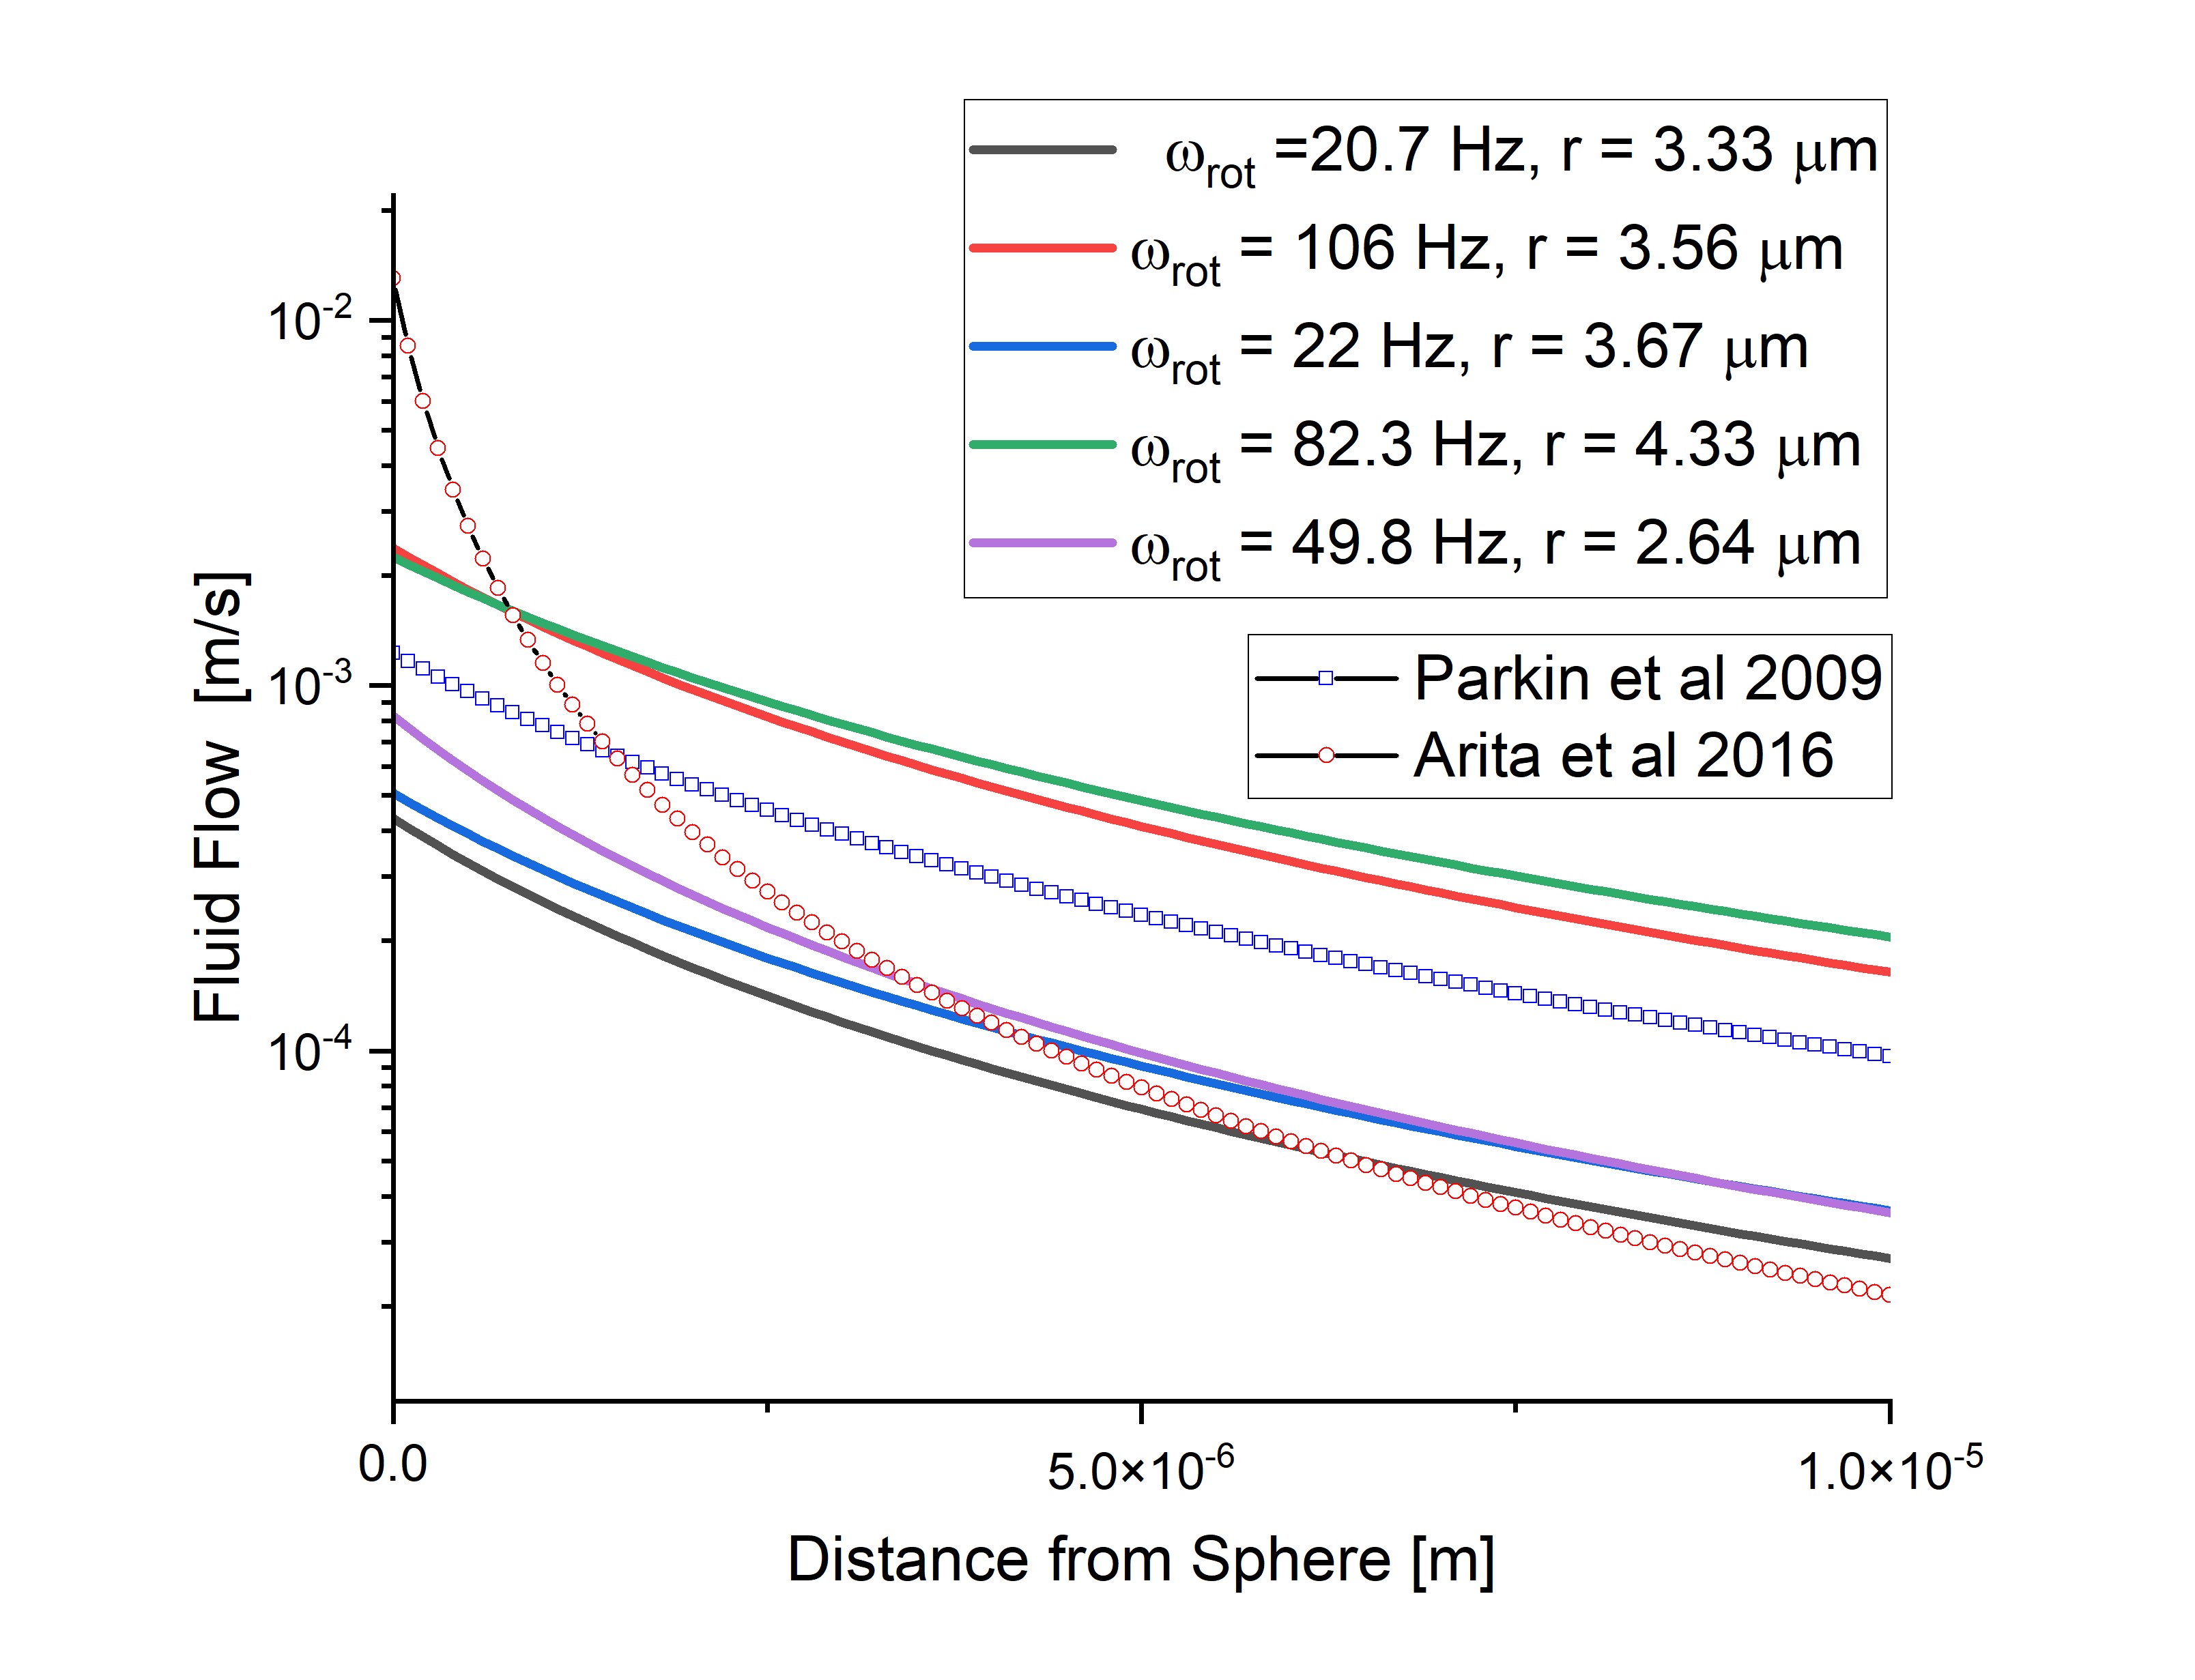
\includegraphics[width=\linewidth]{vaterite_fluid_flow.png}
		\subcaption{}
	\end{subfigure}
	\begin{subfigure}{0.5\linewidth}
		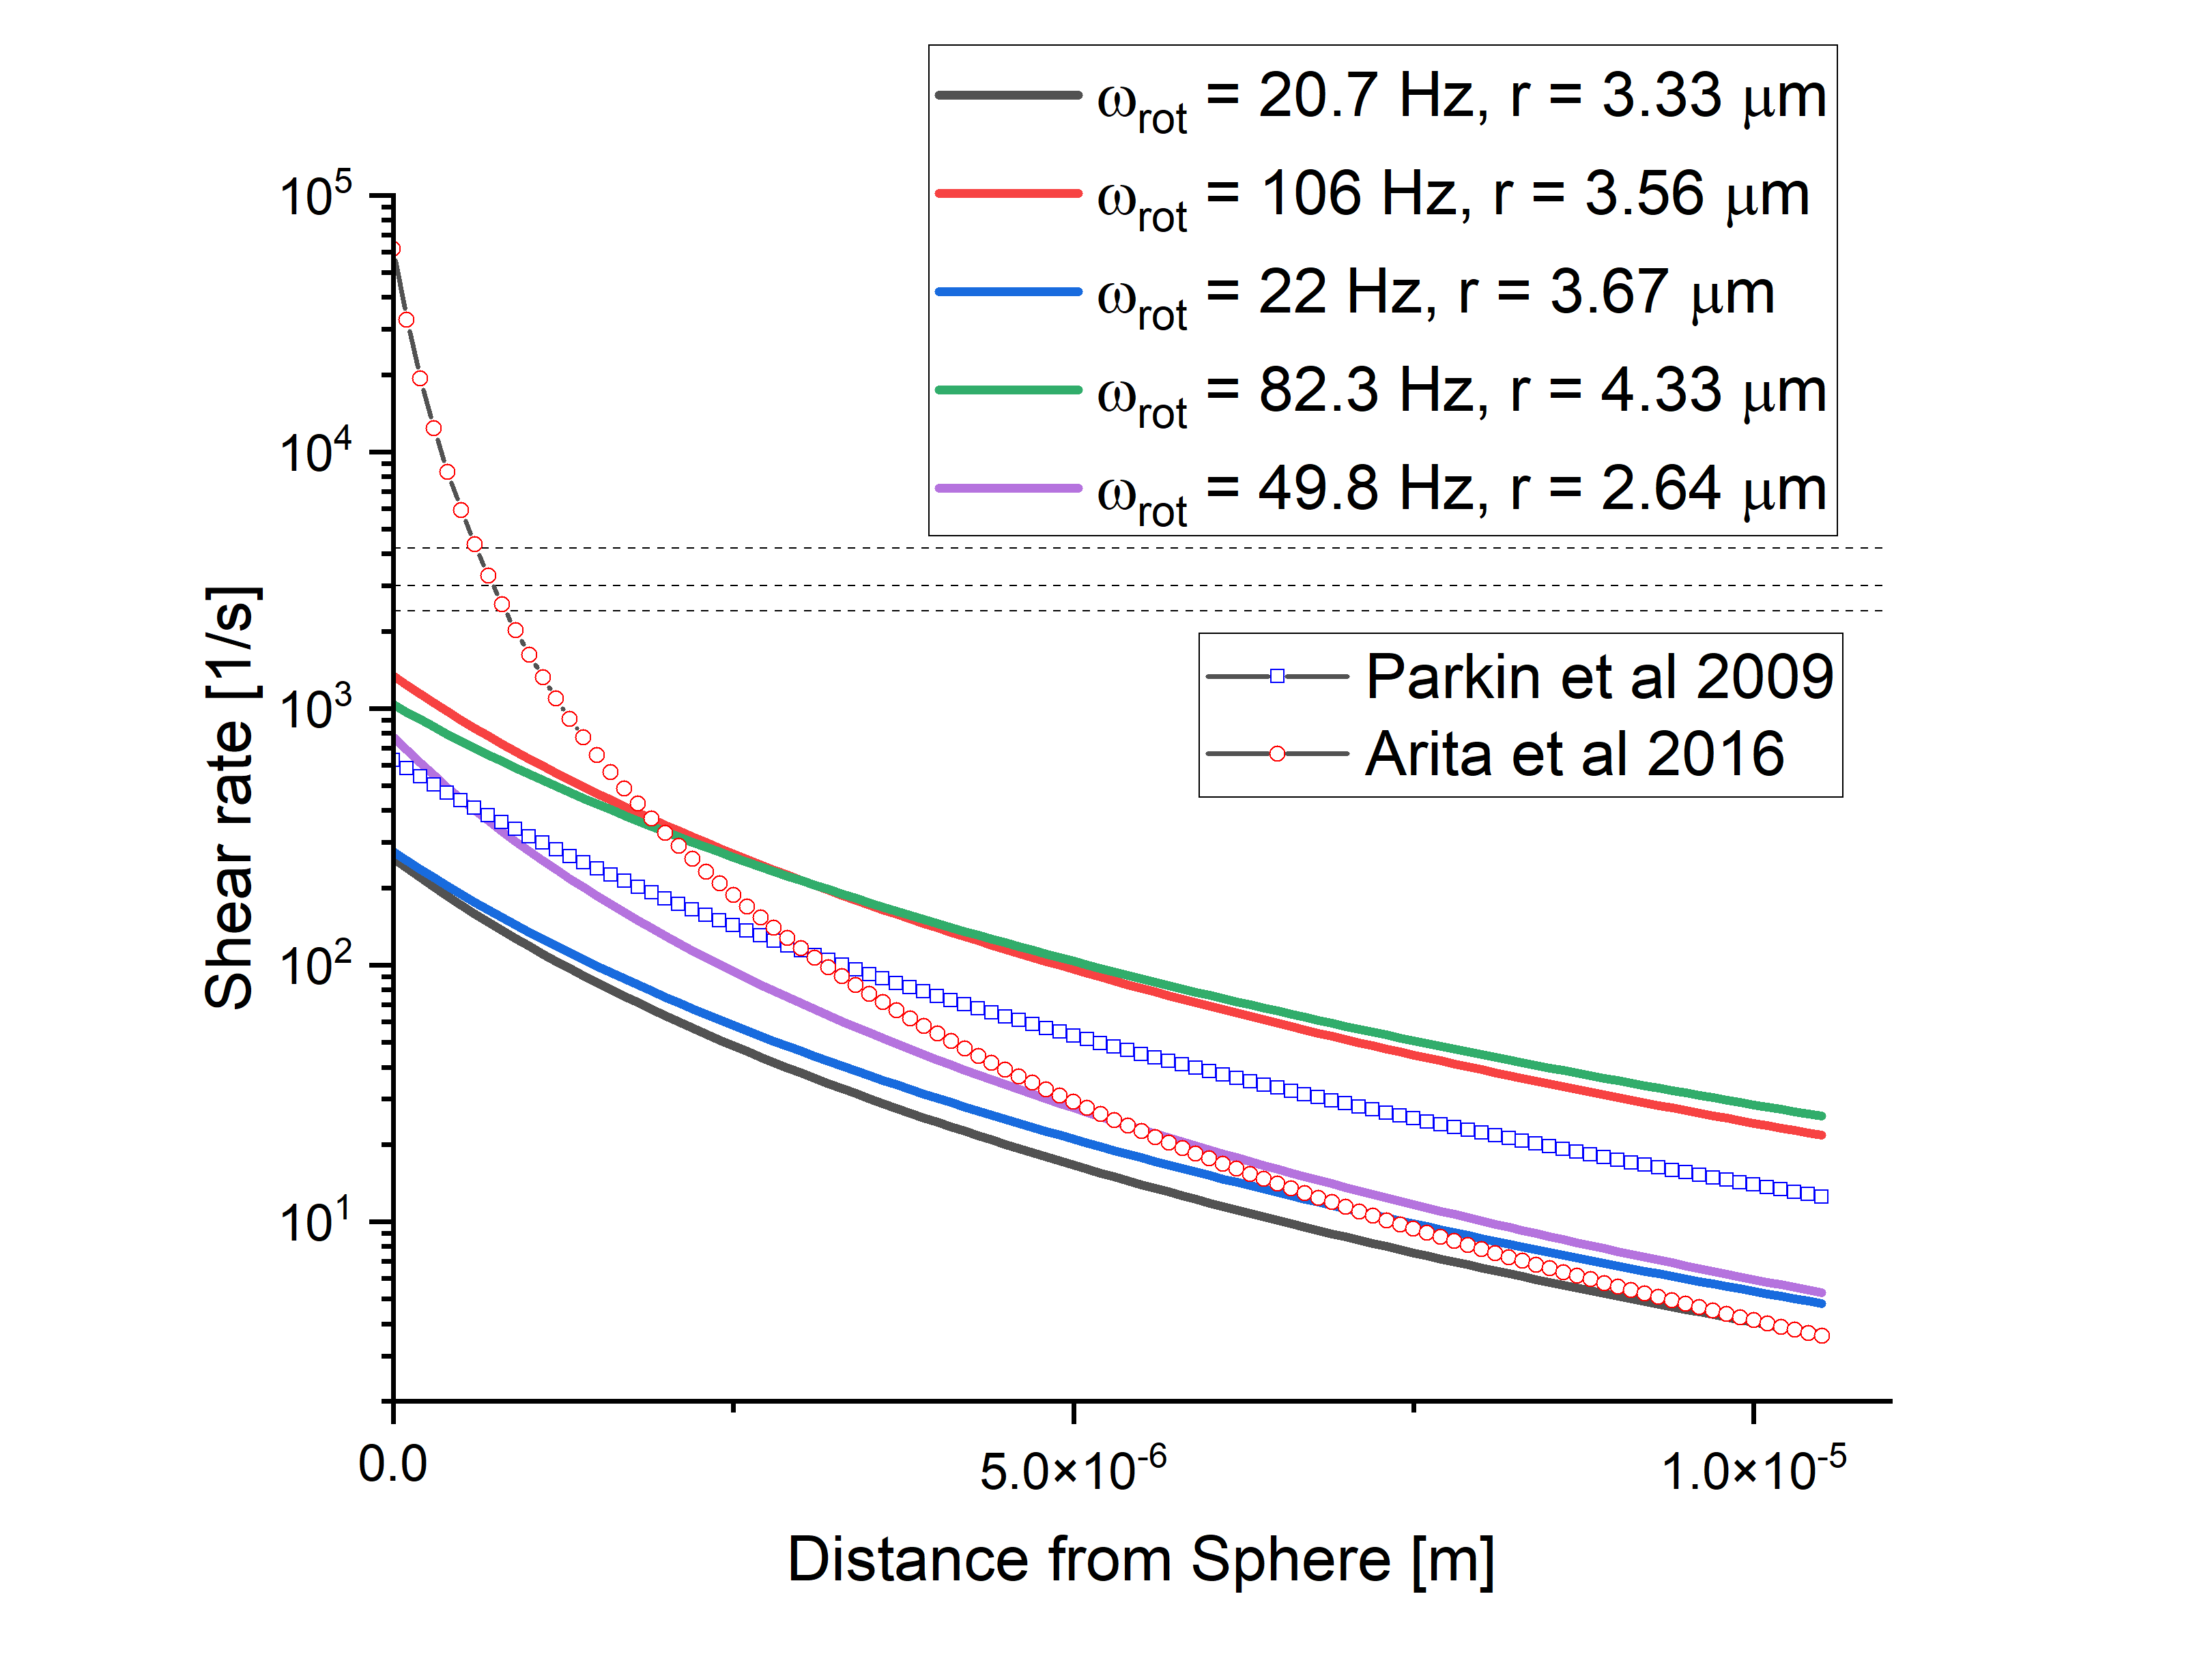
\includegraphics[width=\linewidth]{vaterite_shear_rate.png}
		\subcaption{}
	\end{subfigure}
	\caption{(a) Fluid flow radiating out from the surface of a rotating vaterite sphere. (b) Shear rates computed using Eq.\ref{eq:birefringent_shear}, optimal shear rate is of $3000 s^{-1}$ is indicated by the dotted line. Vaterite radii and rotation frequencies are shown, the laser power was kept constant at 450 mW. Reported rotation rates, and their corresponding fluid flow and shear rates, for vaterite are also plotted alongside lab results.}
\end{figure}

From Fig.\ref{fig:vaterite_shear} it's clear that 

Using a galvano mirror can A particle's motion can be precisely controlled For a simple circular path one can estimate the sphere's speed by the radius of its path and the frequency of its orbit $U = R\omega$; however for a more complex path, such as an elliptical orbit the curve needs to be parametrised. One can describe the position parameter of an ellipse as such:

\begin{align}
	r(u) = \left[acos(2\pi u),bsin(2\pi u), 0 \right]
\end{align}

where a and b are the different characteristic radii of an ellipse, if we assume that u describes time from some initial point we can say $u=t\omega$ where omega is the frequency of orbit. Subbing this in and then taking the partial derivative of position gives:

\begin{align}
	v(t) = \frac{dr(t)}{dt} = \left[-2\pi a\omega \ sin(2\pi t\omega),\ 2\pi b\omega \ cos(2\pi t\omega),0 \right]
\end{align}

In order to compute U we simply take the magnitude of our velocity. For low velocities the fluid flow around the entire sphere can be computed based on the sphere's velocity.

\begin{align}
	u_r(r)=-v(t)cos(\theta)\left(1-\frac{3R}{2r}+\frac{R^3}{2r^3}\right)
\end{align}

Where $\theta$ is the angle from the direction of movement to the point you wish to measure, and $r$ is the radial distance to that point. Again taking the partial derivative we can get the shear rate for a particle moving through the fluid:

\begin{align}
	\dot{\gamma}(r) = \left| \frac{\delta u_r(r)}{\delta r}\right| = v(t)cos(\theta)\left(\frac{3R}{r^2} -\frac{2R^3}{r^4} \right)
\end{align}

Silica beads ($r=1,57 \mu m$) were trapped and moved along an elliptical path

\bibliographystyle{ieeetran}
\bibliography{thesis_bib}

\end{document}